%% This document was written by Sofi�a JIJON 
%% iPLESP
%%
%% Paris, 2017-2018.
%%________________________________________________________________________
\documentclass[12pt]{article}

\usepackage[a4paper, vmargin=3cm, hmargin=3cm]{geometry}
\usepackage{setspace} 	\linespread{1.5}							% Interlinear space
\usepackage[latin9]{inputenc}
\usepackage[T1]{fontenc}
\usepackage[english]{babel}
\usepackage{amsmath,amssymb,amsthm}
%\usepackage[colorlinks=true,linkcolor=black,citecolor=black, urlcolor=black]{hyperref}
\usepackage[colorlinks=true,linkcolor=MyBlue,citecolor=MyBlue, urlcolor=MyBlue]{hyperref}
\usepackage[usenames,dvipsnames,table]{xcolor}
\usepackage{graphicx,float}
\usepackage[sort&compress,square,numbers]{natbib}				% Biblio
\usepackage[labelfont=bf,width=0.9\textwidth,footnotesize]{caption} 		% Use centerlast to center last line.

\newcommand{\figref}[1]{\hyperref[#1]{figure~\ref{#1}}}
\newcommand{\secref}[1]{\hyperref[#1]{section~\ref{#1}}}
\definecolor{MyBlue}{RGB}{0,120,155}
%%
%% Abstract: 300 words
%% Main text: 2500 to 3000 words
%%
%% WORDCOUNT:
%%
%% Abstract: 		 	222
%%
%% Intro: 			 	426
%% Interdisciplinary: 	692
%% My thesis: 			1193
%% Conclusions: 		450
%%------------------------------------------------------
%% TOTAL: 			2761
%%
%%________________________________________________________________________
%%
%%	DOCUMENT
%%________________________________________________________________________
\begin{document}
%%_____________________________________________
%%
%%	Title
%%_____________________________________________
\begin{center}
	{\textcolor{MyBlue}{\huge Interdisciplinary Note  \\ \medskip \large R\'eseau Doctoral en Sant\'e Publique }} \\ 
	\vspace{10pt}
%	{\large \guillemotleft~Prevention of infectious diseases: a game-theoretic approach~\guillemotright}\\ 
	{\large \guillemotleft~Prevention of infectious diseases : from a game-theoretic \\ approach to a multi-level, interdisciplinary perspective~\guillemotright}\\ 
	\vspace{10pt}
	{Sof\'ia JIJ\'ON ALB\'AN}\\ \smallskip
	{\small September, 2019}
\end{center}
%\vspace{2pt}
%%_____________________________________________
%%
%%	Abstract
%%_____________________________________________

\begin{center}
\begin{minipage}{\linewidth}
\rule{\linewidth}{0.2pt}
\vspace{-30pt}

\subsection*{Abstract}
{\small
Despite great efforts and improvements, the prevention of infectious diseases remains a key public health challenge. When facing an ongoing epidemic, individuals may decide to use prevention, or else to get treated in the case of acquiring the infection. Whereas treatment is generally well accepted by infected individuals, the acceptability of prevention may vary between individuals. The individual's perception of the risk of infection, as well as weighing the perceived pros and cons of prevention versus treatment, may lead individuals to adopt preventive behaviors that differ from the public health authorities' recommendations.\medskip

My doctoral research concerns the mathematical modeling of infectious diseases transmission, taking into account individuals' decision-making on the adoption of prevention to avoid the infection during an ongoing epidemic, in the context where efficient treatment is available. We aim to determine whether and under what conditions could voluntary prevention avert an epidemic. Two applications are explored: voluntary vaccination in the context of treatable childhood infectious diseases; and the voluntary use of pre-exposure prophylaxis to avoid HIV infection, by the individuals who are most at risk of infection, among the population of men who have sex with men.\medskip

The purpose of this note is to place my doctoral research project within a broader, interdisciplinary context, from a public health perspective.
}

\paragraph{Keywords:} {infectious diseases; behavioral epidemiology; voluntary prevention; mathematical modeling; game theory.}\\
\rule{\linewidth}{0.2pt}
\end{minipage}
\end{center}
%\vspace{2pt}
%%_____________________________________________
%%
%% ToC
%%_____________________________________________
{
%\newpage
\small
\linespread{0.5}{
\tableofcontents
}
}
%%________________________________________________________________________
%%
%% 	1.  Intro
%%________________________________________________________________________
%\newpage
\section{Introduction}
\subsection*{The \textit{prevention versus treatment} dilemma}

The individual's decision-making on whether or not to adopt prevention methods to avoid infections in a context where efficient treatment is available is known as an individual-level dilemma of \textit{prevention versus treatment}, and remains a subject of debate~\cite{Bosworth2010,Meertens2013}. The individuals' perception on the subject may differ from the public health authorities' recommendations. For instance, despite vaccination promotion, vaccine hesitancy may result in a decline in vaccination coverage~\cite{Larson2014}, reaching sub-optimal levels and thus leading to outbreaks of infectious diseases otherwise controlled~\cite{Jansen2003,Strebel2013}. 

When facing an ongoing epidemic, individuals decide whether or not to use a preventive method by evaluating their risk of infection, its consequences, the availability of both preventive and therapeutic tools, and their related benefits and constraints. Therefore, the individuals' decision on whether or not to adopt a prevention method to avoid the infection may be biased, yet closely related to the course of the epidemic. Indeed, the risk of infection depends on the disease's prevalence, which in turn depends on the effectiveness and coverage of the preventive and therapeutic methods. Hence, each individual's decision may be indirectly influenced by the others' decisions, since the sum of all decisions determines the voluntary prevention coverage, which impacts the epidemic's progression. 

It is thus essential to account for individuals' decision-making on whether or not to adopt a preventive method, in order to evaluate the impact of voluntary prevention on an epidemic. This is the main objective of my doctoral project. The first part of my thesis~\cite{Jijon2017} focuses on the the use of vaccination to prevent treatable childhood infectious diseases. The second part~\cite{Jijon2019} concerns the use of pre-exposure prophylaxis (PrEP) as a prevention method against HIV infection among men who have sex with men (MSM) at high risk of infection, in high-income settings and in the current context of the HIV epidemic, where efficient antiretroviral therapies (ART) are available. Given the focus of my doctoral project, most of the discussion and references presented in this note are about prevention through vaccination and PrEP, but our results may shed some light on many other treatable and preventable infectious diseases.

This note is organized as follows. In \secref{sec:InterdisciplinaryContext}, I place the subject of voluntary prevention within a boarder, interdisciplinary context, from a public health perspective, by identifying the roles of some of the different actors directly related to this public health issue. In \secref{sec:MyThesis}, I present a brief description of my doctoral research, in order to introduce the contribution of my work to the field. Finally, in \secref{sec:Conclusions}, I extend a brief  discussion on the subject's further challenges. 

%%________________________________________________________________________
%%
%% 	2. The interdisciplinary context of the subject
%%________________________________________________________________________
\section{The prevention of infectious diseases: an interdisciplinary challenge}
\label{sec:InterdisciplinaryContext}
Controlling an epidemic is a multi-level, interdisciplinary challenge. The decision-making on whether or not to use prevention is done at the individual level, whereas the preventive method implementation and its impact may be evaluated at the populational level. Public health authorities' recommendations rely on evidence and studies from the scientific community. Public policies are established under limited resources allocated through economical analyses. Finally, prevention promotion and prevention programmes require the active participation of the the media and the general population. 

%%
%%_____________________________________________
%%
\subsection{Public health authorities}
Public health authorities may facilitate access to information and epidemiological data about infectious diseases and the available preventive and therapeutic methods and programmes. In addition, public health authorities need to address the subject of prevention hesitancy~\cite{Larson2016} and difficulties in its accessibility, in order to improve prevention coverage. Reducing the perceived prevention-related barriers~\cite{Larson2014,Jarrett2015,Coleman2017} (which involve monetary and non-monetary aspects), may encourage individuals to adopt preventive methods against infectious diseases and thus, yielding broad prevention uptake. In addition, monetary and/or non-monetary incentives may be used as strategies to improve prevention uptake~\cite{Jarrett2015}.
%%
%%_____________________________________________
%%
\subsection{The participation of the community}
The risk perception as well as the acceptability of prevention may vary between individuals~\cite{Larson2014,Blumenthal2019}. Hence, it is essential for individuals to have a fair perception of their risk of infection, to follow the public health authorities recommendations and reach the health facilities that offer prevention interventions that suit them the best.

Prevention programmes may be importantly reinforced by the participation and support of the community~\cite{ConcertationFR2016}. Unfortunately, the community could also play the role of a barrier against prevention efforts, in the cases where individuals may be susceptible to peer-pressure and social stigma (for instance, HIV-related stigma impacting PrEP acceptability~\cite{Young2014} and peer-pressure against vaccination~\cite{Larson2014}). 

%%
%%_____________________________________________
%%
\subsection{Economical decisions}
Prevention has shown to be cost-effective, with respect to treatment, for infectious diseases such as measles~\cite{Strebel2013}, HIV~\cite{Cambiano2018}, influenza~\cite{Dabestani2019} and other emerging infectious diseases~\cite{Heymanng2014}. These results place prevention as a public health priority regarding ressources allocation.

Affordability and accessibility being key aspects in prevention adoption, it is also important to highlight the necessity of reducing socio-economical inequalities. For instance, income has been identified as a factor impacting vaccination acceptability~\cite{Larson2014}, and gaps still remain in the path to HIV elimination at the global scale, given that only 1 out of 10 MSM has access to HIV prevention interventions~\cite{WHO_Gap}. %Integrating PrEP into routine preventive health (instead of targeted programmes) may help avoid exacerbating disparities~\cite{Calabrese2017}.
%%
%%_____________________________________________
%%
\subsection{Mathematical epidemiology}
The mathematical modeling of infectious diseases has become a key tool for epidemiology, helping understanding epidemics' dynamics, estimating the values of parameters not directly measurable, predicting future states of the system and selecting optimal intervention designs~\cite{Brauer2017}.

Disease transmission has been mostly studied using compartimental models~\cite{Brauer2017,Rohani2008}, which allow to study the epidemic dynamics at the population level, by tracing the transition of individuals trough different states, regarding the infection. Recently, individual behavior and its impact on epidemic dynamics has also been introduced in the modeling of infectious diseases prevention~\cite{Verelst2016}. For instance, game-theoretic approaches have been used. Game theory allows, among other things, to model rational individual's decision-making and strategies. Hence, game-theoretic models allow to include strategic individual-level decision-making on whether or not to adopt a preventive method to avoid the infection. 

Mathematical models are useful when they are adapted to the research question and its context. Therefore, modelers need to find the right balance between the complexity that helps increasing model accuracy, and the simplicity that allows a model to clearly be understood, to be flexible and to be solved without requiring high levels of computing power~\cite{Rohani2008}. In addition, models are parametrized using available data, which highlights the importance of good-quality of data collection.
%%
%%_____________________________________________
%%
\subsection{Scientific communication}
The dissemination of information about epidemics and disease burden may shape individual's sense of their risk of infection, as well as provide awareness on the available preventive and therapeutic tools. It is thus essential to account for the impact of scientific communication within public prevention efforts. Unfortunately, there is evidence of misinterpretation of research results spreading through mass media~\cite{Haneef2015}.

For individuals to make well-informed decisions, it is important, on the one hand, that researchers communicate their results in the most efficient way possible so misinterpretations are reduced to a minimum; on the other hand, that media transmit scientific results accurately. For instance, explaining the meaning of prevention-parameters estimations, such as the preventive method effectiveness may help broaden prevention rollout programmes~\cite{Underhill2016}.  

%%________________________________________________________________________
%%
%% 	3. My thesis
%%________________________________________________________________________
\section[The contribution of my doctoral research project]{The contribution of my doctoral research project}
\label{sec:MyThesis}

My doctoral research is entitled \textit{``Prevention of infectious diseases: a game-theoretic approach''}. The main objective is to model the transmission of infectious diseases taking into account the individuals' decision-making on the adoption of prevention methods in order to avoid infection during an ongoing epidemic, in the context where efficient treatment is available, in high-income settings. In particular, we intend to determine whether and under which conditions could the voluntary use of prevention alleviate   (that is, reduce the number of infections) and/or eliminate an epidemic.

\subsection{Modeling the voluntary prevention of treatable infectious diseases}
We propose a mathematical model describing the interaction between voluntary prevention and epidemic dynamics. To describe the disease transmission among the population, we use a deterministic compartmental model, defined by a system of ordinary differential equations. To describe the individual's decision-making on whether or not to adopt a preventive method, we rely on a game-theoretical approach: a non-cooperative single-player game. A depiction of the model is shown in~\figref{fig:ModelDiagram}. 

\begin{figure}[H]
	\centering	
	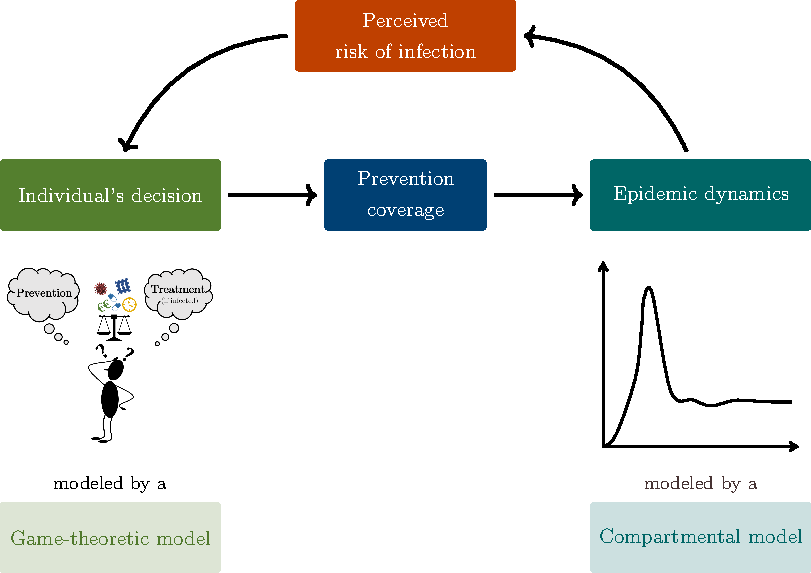
\includegraphics[width=0.85\linewidth]{Fig_ModelDiagram}
	\caption[Diagram of the mathematical model]{{\bf Diagram of the mathematical model\\}
	\small Depiction of the interaction between voluntary prevention and epidemic dynamics. Each individual makes a decision on whether or not to adopt a preventive method to avoid the infection. Then, the sum of all individuals' decisions determines the voluntary prevention coverage, which (along with other factors such as prevention effectiveness and treatment coverage) affects the epidemic dynamics. In turn, the state of the epidemic provides the individuals a perception of the probability of infection, which will be acknowledged in the decision-making on whether or not to adopt the preventive method. The individual-level decision-making is modeled using a non-cooperative single-player game, while the infectious disease transmission at the populational level is modeled using a deterministic compartmental model.
	}
	\label{fig:ModelDiagram}
\end{figure}

Our approach assumes that individuals address the prevention versus treatment dilemma by developing a sense for their risk of infection, its consequences, the availability of both preventive and therapeutic tools, and their relative benefits and constraints (e.g., undesired secondary effects, price, reimbursement policies, accessibility, disease morbidity, etc.). In a game theoretic framework, these factors are considered as \textit{cost}. An individual's expected utility can thus be expressed as a function of the relative cost of prevention versus treatment and the probability of acquiring infection, perceived by the individual. %Game theory postulates that the individual-level decision-making maximizes the utility of prevention versus treatment. 

The prevention coverage that maximizes the utility yields the probability for an individual to adopt the prevention method as a function of the model parameters, which we refer to as the \textit{voluntary prevention coverage}. In particular, we study the voluntary prevention coverage in terms of the relative cost perceived by individuals.

\subsection{Exploring two applications}
My doctoral research consists of two applications of this method. First, we studied voluntary vaccination in the context of treatable childhood infectious diseases (see~\secref{Project_Vaccination} and~\cite{Jijon2017}). Then, a second application concerns the HIV epidemic and the voluntary use of pre-exposure prophylaxis (see~\secref{Project_PrEP} and~\cite{Jijon2019}). 

%The results from the first project were obtained analytically, constituting a theoretical basis for the second project, which was implemented numerically. 


%%_____________________________________________
%%
%%	3.1. Vaccination
%%_____________________________________________
\subsubsection{The voluntary vaccination against childhood infectious diseases} \label{Project_Vaccination}

The first part of my doctoral research was devoted to the analysis of voluntary vaccination in the context of treatable childhood infectious diseases that are preventable by vaccination. We assumed that immunization was imperfect by two means: the effectiveness of the vaccine was not complete (that is, a proportion of the population was not protected against the disease after vaccination) and the vaccine-induced immunity was of limited duration.

Our results~\cite{Jijon2017} suggest that imperfect prevention methods may nevertheless avert epidemics. We obtained the effective vaccination coverage, expressed as a function of the relative cost of prevention versus treatment and we identified three behaviors. First, if the relative cost is too high, individuals do not get vaccinated. Second, if the relative cost is moderate, some individuals get vaccinated and voluntary vaccination alleviates the epidemic. In this case, the vaccination coverage grows steadily with decreasing relative cost. Unlike previous studies~\cite{Bauch2004}, we found a third case, where voluntary prevention may avert the epidemic, provided that the relative cost is sufficiently low.  In addition, we found that epidemic elimination is only possible if the immunity offered by vaccination is long-lasting. 

However, disease elimination is only temporary: with increasing perceived cost of vaccination versus treatment, vaccination coverage may reach suboptimal levels again. Indeed, when the vaccination coverage is high enough to control the epidemic, individuals no longer perceive the morbidity and mortality associated with the disease, and controversies about the safety of the vaccine may emerge. This may change the perception of the cost of prevention versus treatment and thus result in a decrease in immunization coverage and the situation may be reversed towards the epidemic status.  Therefore, maintaining a perceived cost of vaccination sufficiently low was identified as a main objective to achieve and maintain disease elimination.

%%_____________________________________________
%%
%%	3.2. HIV & PrEP
%%_____________________________________________
\subsubsection{The voluntary use of pre-exposure prophylaxis to prevent HIV infection} \label{Project_PrEP}
The second part of my doctoral research was devoted to the modeling of HIV transmission within the population of men who have sex with men (MSM), taking into account the individual-level decisions on whether or not to adopt PrEP as a prevention method against HIV, in the current therapeutic context, where effective ART are available. In particular, we addressed this subject within one of the most at risk populations in mainland France: MSM in �le-de-France~\cite{Jijon2019}.

Despite the efforts to prevent and treat HIV infection, the epidemic continues to spread globally. In most high-income countries, the highest number of infections remains identified among MSM~\cite{WHO_KeyPop2016}. PrEP consists of the use of ART by uninfected individuals before the exposition to HIV. Its effectiveness among MSM has been estimated at 86\%~\cite{Molina2015}, which places PrEP among the most effective HIV prevention methods~\cite{WHO_ART2016}. Therefore, PrEP is currently recommended for MSM as a prevention method against HIV~\cite{WHO_KeyPop2016,WHO_ART2016}.

Mathematical modeling has been extensively used to describe the HIV epidemic among MSM and to evaluate the impact of preventive interventions on the epidemic's dynamics~\cite{Punyacharoensin2011}. Studies have evaluated the impact of a PrEP rollout on the HIV epidemic among MSM, predicting a remarkable reduction in the number of HIV infections and even the epidemic elimination~\cite{Rozhnova2018}. However, to the best of our knowledge, no study has addressed the individual-level decision-making on whether or not to adopt PrEP to avoid HIV infection and thus evaluated the impact of voluntary adoption of PrEP on the HIV epidemic. This constituted our main objective. 

We developed a model for the transmission of HIV among the population of sexually active MSM~\cite{Jijon2019}. We stratified the population by the individuals' risk of infection. Only individuals at high risk of infection were eligible to take PrEP. Individuals were assumed to have a fair perception of their risk of infection, but other scenarios, where individuals misperceive their risk of infection, were also considered.

We obtained the voluntary PrEP coverage as a function of PrEP effectiveness and the relative cost of PrEP versus ART~\cite{Jijon2019}. Four behaviors of the voluntary PrEP coverage were identified. First, nobody uses PrEP because PrEP effectiveness is too low and/or relative cost perceived by the individual is too high. Second, all individuals are willing to adopt PrEP because the relative cost is low, but PrEP effectiveness is too low to eliminate the epidemic. Third, some but not enough individuals decide to use PrEP because the relative cost is moderate and thus, the epidemic is alleviated but not eliminated. And fourth, high levels of PrEP coverage are reached because relative cost is low and PrEP effectiveness is high and thus, the epidemic may be averted. 

According to our findings~\cite{Jijon2019}, disease elimination may be only temporary: epidemic status may be reached again if PrEP coverage decreases (either because PrEP cost is again perceived as high, or because PrEP effectiveness decreases due, for instance, to a decrease in PrEP adherence). A PrEP program targeting the individuals most at risk may eliminate the HIV epidemic at the population level in the long term, provided that individuals have a fair risk perception and the perceived cost of PrEP is maintained low.

Reducing the cost of PrEP perceived by high-risk MSM may involve not only the reduction of the price of PrEP but also the reduction of other barriers, such as: difficulties regarding PrEP uptake and accessibility, undesired secondary effects, social stigma and discrimination~\cite{Arnold2016,Thomann2017,Bull2018,Gilson2018}.

%A scientific article presenting our methods and findings has been recently submitted for publication~\cite{Jijon2019}.

%%________________________________________________________________________
%%
%% 	4. Conclusions
%%________________________________________________________________________
\section{Conclusions} \label{sec:Conclusions}
Our results suggest that the voluntary adoption of preventive methods may avert epidemics. Along with high levels of protection offered by the preventive methods, it is essential to maintain a low perception of the cost of preventive methods against infectious diseases in order to reach and maintain a coverage level ensuring epidemic elimination. Hence, public health authorities need not only to establish prevention programmes, but also to promote and maintain them, in the long run. 

In the case of childhood vaccination~\cite{Jijon2017}, we believe some interventions could be implemented to increase vaccination coverage in high-income settings: i) the incentive by reducing the price of health insurance premiums as the vaccination calendar is respected and completed; ii) sharing the success of prevention programmes in the media, and iii) the promotion of a fair perception through the continuous recall of epidemiological data on vaccine-preventable diseases and their consequences in terms of morbidity and mortality, in parallel with a clear information about the adverse effects of vaccination and treatment.

In the case of PrEP uptake among the MSM community, the perceived cost of PrEP need to be importantly decreased to achieve levels of PrEP coverage that may lead to HIV-epidemic elimination. For instance, by increasing accessibility to broadly provide PrEP through public health programmes. We also found that a fair perception of the own risk of infection is essential for making more room for prevention programmes to aim epidemic elimination through cost reduction~\cite{Jijon2019}.
 
According to our findings, public health programmes aiming epidemic elimination may ensure high prevention coverage ---yielding epidemic elimination--- by maintaining a low cost of the preventive method perceived by individuals. The cost involves not only the monetary aspects, but also all the difficulties and discomfort individuals may experience thorough the adoption of preventive methods. Therefore, the reduction of the perceived cost of prevention may be pursued from different perspectives at a different levels, requiring joint efforts from different disciplines. 

In addition, a voluntary-prevention-adoption approach relies on the information that individuals will weigh in their decision-making. Therefore, it is essential for individuals to be fairly informed about the risk of infection and the consequences of the different strategies they could adopt. Accurate information shared through social media about the current status of the epidemic, fighting against social stigma, and offering opportunities for the community to be involved in the preventive efforts are some of the ways that the population may play an essential role towards epidemic elimination. 

We hope our approach, which includes the individuals' decision-making component to a classic transmission model, may yield new insight into the impact of prevention on the epidemic in the context of other infectious diseases such as Hepatitis B, human papillomavirus, Hepatitis C, syphilis, influenza, etc. 
 
%%________________________________________________________________________
%%
%% 	REFERENCES
%%________________________________________________________________________
%%
%% Max 30 Refs.
%%
%	\newpage
	\vspace{-24pt}
	\renewcommand{\refname}{\section{References}}
%	\addcontentsline{toc}{section}{References}
%	\nocite{*} 					% Uncomment so all the references in the .bib (even those who were not cited) are included
	\small
%	\footnotesize
	\bibliographystyle{TheseBib} 	% use abbrvnat for abbreviated first name unsrtnat
	\bibliography{Biblio_NID}
\end{document}

